\chapter{约化态、纠缠熵与幺正演化}

密度矩阵最初是作为不完全制备的自然描述而出现的：一个量子系统已被制备，但我们并不确切知道它是如何被制备的。纠缠赋予同一个数学对象以更深刻的角色。即便复合系统的态被完全知晓，其子系统一般也没有属于自己的态矢量。它的约化密度矩阵包含了所有能在局部被预测的信息。我们将用分量推导这一论断，在两个自旋态上检验它，并用熵来区分乘积态与纠缠态。随后我们将转向第二个问题：量子态如何随时间变化。内积的保持将引出幺正性、厄米生成元以及Schr\"odinger方程。

\section{密度矩阵与不完全制备}

假设一个电子被置于强磁场中并允许其沿磁场方向排列。另一个人选择了磁场方向并制备了这个电子，但没有告诉我们该方向。因此，尽管我们不知道自旋处于哪个态，它仍可能处于一个完全确定的纯态。我们可能知道关于各种可能制备方式的概率分布，也可能一无所知。密度矩阵\(\rho\)正是对这类不完全信息的量子描述。

经典类比是相空间上的概率密度，或离散构型上的概率分布。量子对象则是一个具有三个基本性质的算符：
\begin{equation}
\rho^\dagger=\rho,
\qquad
\operatorname{Tr}\rho=1,
\qquad
\lambda_i\geq 0,
\end{equation}
其中\(\lambda_i\)是\(\rho\)的本征值。厄米性使本征值为实数，并提供一组正交归一本征基。正定性使它们成为可容许的概率，而归一化给出
\begin{equation}
\sum_{i=1}^{n}\lambda_i=1.
\end{equation}
在\(\rho\)的本征基中，\(\lambda_i\)是赋予第\(i\)个本征态的概率。

完全无知的情形是希尔伯特空间中没有任何方向被偏爱：
\begin{equation}
\rho_{\mathrm{max}}=\frac{1}{n}I.
\end{equation}
每个本征值都是\(1/n\)。在相反的极端，完全知识由归一化态\(\ket{\psi}\)表示，即
\begin{equation}
\rho_\psi=\ket{\psi}\bra{\psi}.
\end{equation}
这是到由\(\ket{\psi}\)张成的一维子空间上的投影算符。

\begin{classroomqa}
\lecturetimestamp{00:06:47}
\audiencequestion{一个制备过程能否被描述为在两个非正交态之间的五五开选择，例如两个自旋方向相隔\(45^\circ\)？}
\lecturerresponse{这样的制备程序是可能的，但这两个权重一般并不是所得密度矩阵的本征值。人们先构造投影算符的加权和，然后将其对角化。本征值那种干净的概率解释属于\(\rho\)的正交归一本征基，而不一定属于制备者所指名的那些非正交态。}
\end{classroomqa}

\begin{classroomqa}
\lecturetimestamp{00:07:47}
\audiencequestion{纯态与混合态的区别是什么？}
\lecturerresponse{纯态的密度矩阵只有一个非零本征值，等于\(1\)。混合态则有不止一个非零本征值。较早的文献使用德语词\emph{Gemisch}；现代术语则直接称为\emph{混合态}。}
\end{classroomqa}

让我们验证纯态投影算符的谱。归一化给出
\begin{equation}
\rho_\psi\ket{\psi}
=\ket{\psi}\braket{\psi}{\psi}
=\ket{\psi},
\end{equation}
所以\(\ket{\psi}\)是一个本征值为\(1\)的本征矢量。若\(\ket{\phi}\)与\(\ket{\psi}\)正交，则
\begin{equation}
\rho_\psi\ket{\phi}
=\ket{\psi}\braket{\psi}{\phi}
=0.
\end{equation}
因此，每个与\(\ket{\psi}\)正交的方向都具有本征值零。

\begin{figure}[htbp]
\centering
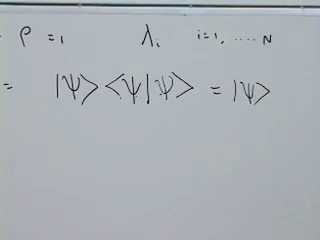
\includegraphics[width=0.72\textwidth]{lecture_08_figure_06.png}
\caption{纯态的密度矩阵起投影算符的作用：\(\rho\ket{\psi}=\ket{\psi}\)。}
\lectureframe{00:09:32}
\end{figure}

\section{由迹求期望值}

密度矩阵的操作规则是
\begin{equation}
\overline{M}=\operatorname{Tr}(\rho M),
\end{equation}
其中\(M\)是一个可观测量。对于两个因子，迹的循环性质给出
\begin{equation}
\operatorname{Tr}(\rho M)=\operatorname{Tr}(M\rho),
\end{equation}
无论\(\rho\)与\(M\)是否对易。

在任意正交归一基\(\{\ket{i}\}\)中，
\begin{equation}
\operatorname{Tr}X=\sum_i\bra{i}X\ket{i}.
\end{equation}
其数值不依赖于基的选择。对于纯态，
\begin{align}
\overline{M}
&=\operatorname{Tr}\!\left(\ket{\psi}\bra{\psi}M\right) \\
&=\sum_i\braket{i}{\psi}\bra{\psi}M\ket{i} \\
&=\bra{\psi}M\left(\sum_i\ket{i}\bra{i}\right)\ket{\psi} \\
&=\bra{\psi}M\ket{\psi}.
\end{align}
而恒等算符的分解
\begin{equation}
\sum_i\ket{i}\bra{i}=I,
\end{equation}
将密度矩阵规则还原为熟悉的纯态期望值。

\begin{figure}[htbp]
\centering
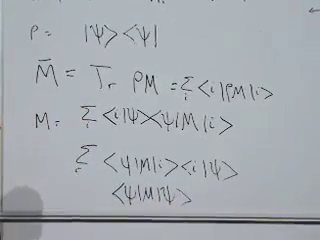
\includegraphics[width=0.74\textwidth]{lecture_08_figure_07.png}
\caption{纯态投影算符的迹计算与恒等算符的分解。}
\lectureframe{00:14:25}
\end{figure}

\begin{classroomqa}
\lecturetimestamp{00:14:38}
\audiencequestion{左边的量应当是\(\overline{M}\)，即\(M\)的平均值吗？}
\lecturerresponse{是的。迹并不是算符\(M\)本身；它是标量期望值\(\overline{M}\)。}
\end{classroomqa}

对于一般的密度矩阵，选取其本征基：
\begin{equation}
\rho\ket{j}=\lambda_j\ket{j}.
\end{equation}
在\(\rho\)与\(M\)之间插入完备态集：
\begin{align}
\overline{M}
&=\sum_i\bra{i}\rho M\ket{i} \\
&=\sum_{i,j}\bra{i}\rho\ket{j}\bra{j}M\ket{i} \\
&=\sum_{i,j}\lambda_j\delta_{ij}\bra{j}M\ket{i} \\
&=\sum_j\lambda_j\bra{j}M\ket{j}.
\end{align}
这是一个普通的加权平均：\(\lambda_j\)是第\(j\)个本征态的概率，而\(\bra{j}M\ket{j}\)是\(M\)在该态中的期望值。

\begin{classroomqa}
\lecturetimestamp{00:18:12}
\audiencequestion{为什么最后一个矩阵元中的两个标签都变成了\(j\)，而哪个指标仍在被求和？}
\lecturerresponse{因为\(\rho\)在此基下是对角的，\(\bra{i}\rho\ket{j}=\lambda_j\delta_{ij}\)，所以只有满足\(i=j\)的项存活。原来的双重求和坍缩为一个求和，可以称之为对\(j\)的求和。哑求和指标的名称没有物理意义。}
\end{classroomqa}

\section{熵作为缺失的信息}

对于经典概率分布\(\{p_i\}\)，定义
\begin{equation}
S=-\sum_i p_i\log p_i,
\end{equation}
其中\(0\log 0\)理解为其极限值\(0\)。若一个概率等于\(1\)而其余全部为零，则\(S=0\)：状态是已知的。若全部\(n\)种可能性等概率，则
\begin{equation}
p_i=\frac{1}{n},
\qquad
S=-n\left(\frac{1}{n}\log\frac{1}{n}\right)=\log n.
\end{equation}
因此，当概率分布扩展到更多显著可能性上时，熵增大。粗略地说，当使用自然对数时，\(e^S\)是权重相当的有效状态数。

\begin{figure}[htbp]
\centering
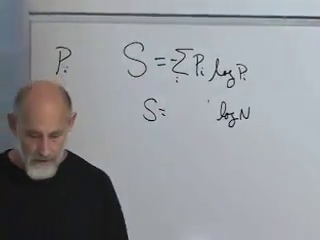
\includegraphics[width=0.68\textwidth]{lecture_08_figure_08.png}
\caption{概率分布的熵与等概率值\(S=\log n\)。}
\lectureframe{00:21:08}
\end{figure}

对于密度矩阵，同样的定义应用于其本征值：
\begin{equation}
S(\rho)=-\sum_i\lambda_i\log\lambda_i
=-\operatorname{Tr}(\rho\log\rho).
\end{equation}
第一个表达式是立即需要的；迹形式强调答案与基无关。

\section{复合系统与局域实验}

考虑两个子系统\(A\)和\(B\)。基矢量写作\(\ket{a,b}\)。若\(A\)有\(N\)个基态而\(B\)有\(n\)个，则复合系统有\(Nn\)个基态。两个系统不必相同：一个可以是二态自旋，另一个可以是三态原子。

这对系统最一般的纯态是
\begin{equation}
\ket{\Psi}
=\sum_{a,b}\psi(a,b)\ket{a,b},
\qquad
\sum_{a,b}|\psi(a,b)|^2=1.
\end{equation}
现在让Alice测量一个仅作用于子系统\(A\)的观测量\(M_A\)。在复合Hilbert空间上，该算符为\(M_A\otimes I_B\)。其矩阵元为
\begin{equation}
\bra{a',b'}M_A\otimes I_B\ket{a,b}
=\bra{a'}M_A\ket{a}\,\delta_{b'b}.
\end{equation}
\(B\)标签是被动的。

将期望值完整写出：
\begin{align}
\expect{M_A}
&=\bra{\Psi}M_A\otimes I_B\ket{\Psi} \\
&=\sum_{a',b'}\sum_{a,b}
\psi^*(a',b')\psi(a,b)
\bra{a'}M_A\ket{a}\delta_{b'b} \\
&=\sum_{a',a,b}
\psi^*(a',b)\psi(a,b)
\bra{a'}M_A\ket{a}.
\end{align}

\begin{classroomqa}
\lecturetimestamp{00:29:12}
\audiencequestion{为什么左矢上的标签带撇而右矢上的不带撇？}
\lecturerresponse{在计算矩阵元之前，左矢和右矢是独立的求和，因此它们需要各自的哑标签。撇号将左矢指标与右矢指标区分开。然后算符和内积决定这些标签中哪些必须相同。}
\end{classroomqa}

保持\(a\)和\(a'\)固定，对\(b\)求和。结果得到子系统\(A\)上的一个矩阵：
\begin{equation}
\boxed{
\rho_A(a,a')
=\sum_b\psi(a,b)\psi^*(a',b)
}.
\end{equation}
这就是\(A\)的约化密度矩阵，等价地，是纯态投影算符对\(B\)的部分迹：
\begin{equation}
\rho_A=\operatorname{Tr}_B\ket{\Psi}\bra{\Psi}.
\end{equation}
局域期望值变为
\begin{equation}
\expect{M_A}
=\sum_{a,a'}\rho_A(a,a')\bra{a'}M_A\ket{a}
=\operatorname{Tr}_A(\rho_A M_A).
\end{equation}

\begin{figure}[htbp]
\centering
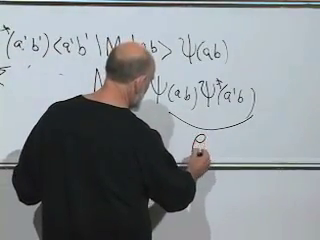
\includegraphics[width=0.76\textwidth]{lecture_08_figure_09.png}
\caption{\(B\)指标被求和掉，留下一个关于两个\(A\)指标的矩阵。}
\lectureframe{00:33:50}
\end{figure}

\begin{classroomqa}
\lecturetimestamp{00:35:39}
\audiencequestion{这个局域可观测量在子系统\(B\)上是否只是恒等算符？}
\lecturerresponse{正是如此。\(M_A\otimes I_B\)可以改变\(A\)坐标，但既不改变\(b\)，也不以其他方式依赖它。这就是为什么它在\(B\)空间中的矩阵元是\(\delta_{b'b}\)。}
\end{classroomqa}


因此，对于局限于\(A\)的实验，所有预测都包含在\(\rho_A\)中。Bob不必测量他的子系统。仅仅是不使用\(B\)自由度，就迫使Alice的描述变为密度矩阵形式。

\section{纯整体可以有混合的部分}

组合系统处于纯态\(\ket{\Psi}\)，然而\(\rho_A\)一般会有多个非零本征值。对整体的完全知识并不意味着每个部分都有一个态矢量。猫和枪可以有一个纠缠态矢量；此时仅猫本身由约化密度矩阵描述。

\begin{classroomqa}
\lecturetimestamp{00:38:25}
\audiencequestion{\(\operatorname{Tr}(M\rho)\)可以被替换为\((\operatorname{Tr}M)(\operatorname{Tr}\rho)\)吗？}
\lecturerresponse{不可以。乘积的迹一般不是迹的乘积。循环性允许\(\operatorname{Tr}(M\rho)=\operatorname{Tr}(\rho M)\)，但它不能将迹分解。}
\end{classroomqa}

\begin{classroomqa}
\lecturetimestamp{00:38:49}
\audiencequestion{我们是从仅有的基态\(\ket{a,b}\)出发，还是从最一般的纯态出发？}
\lecturerresponse{从复合系统最一般的纯态出发：\(\ket{\Psi}=\sum_{a,b}\psi(a,b)\ket{a,b}\)。单个\(\ket{a,b}\)只是一个基矢量。令人惊讶的是，即使这个完全确定的复合矢量也能给出混合的约化态。}
\end{classroomqa}

与经典力学的对比十分鲜明。关于复合系统的完整经典信息确定了它的每个坐标，因而也确定了每个子系统。经典概率分布当然可以被边缘化，但如果原分布集中在一个相空间点上，那么每个边缘分布也都集中在一个确定值上。量子纯态则不必具有这一性质。

\begin{classroomqa}
\lecturetimestamp{00:40:46}
\audiencequestion{对\(B\)求和与对经典位置--速度分布关于速度积分有何不同？}
\lecturerresponse{这些操作看起来相似，但它们的纯态极限不同。一个完全已知的经典相空间点同时确定了位置和速度，因此任一边缘分布都保持确定。一个完全已知的纠缠量子态却可以给任一子系统一个非平凡的混合态。因此，偏迹揭示了经典中“纯整体蕴含纯部分”这一蕴含关系在量子情形下的失效。}
\end{classroomqa}

\section{乘积态：例外情形}

\(\rho_A\)何时保持纯态？答案是波函数必须因子化：
\begin{equation}
\psi(a,b)=\phi(a)\chi(b).
\end{equation}
假设\(\phi\)和\(\chi\)分别归一化。代入约化密度矩阵得到
\begin{align}
\rho_A(a,a')
&=\sum_b\phi(a)\chi(b)\phi^*(a')\chi^*(b) \\
&=\phi(a)\phi^*(a')\sum_b|\chi(b)|^2 \\
&=\phi(a)\phi^*(a').
\end{align}
因此
\begin{equation}
\rho_A=\ket{\phi}\bra{\phi}.
\end{equation}
它有一个本征值\(1\)，其余所有本征值均为\(0\)，熵为零。

\begin{figure}[htbp]
\centering
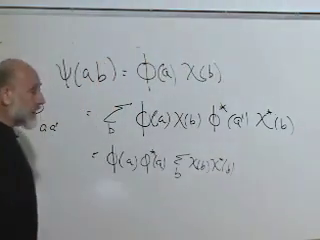
\includegraphics[width=0.74\textwidth]{lecture_08_figure_10.png}
\caption{对于因子化的波函数，对\(B\)的求和归结为\(\chi\)的归一化。}
\lectureframe{00:46:35}
\end{figure}

\begin{classroomqa}
\lecturetimestamp{00:44:17}
\audiencequestion{\(\phi(a)\)本身就是\(A\)系统的态吗？}
\lecturerresponse{它是该态的波函数分量。更明确地说，\(\ket{\phi}=\sum_a\phi(a)\ket{a}\)，类似地\(\ket{\chi}=\sum_b\chi(b)\ket{b}\)。因子化意味着\(\ket{\Psi}=\ket{\phi}\otimes\ket{\chi}\)，即一个在\(A\)与\(B\)之间没有纠缠的乘积态。}
\end{classroomqa}

对于每个局域可观测量，
\begin{equation}
\expect{M_A}
=\operatorname{Tr}(\rho_A M_A)
=\bra{\phi}M_A\ket{\phi}.
\end{equation}
子系统\(A\)的行为恰好如同一个纯态\(\ket{\phi}\)。因此，对于双分体纯态，\(\rho_A\)的熵检验了乘积结构：为零意味着乘积态，而非零熵意味着纠缠。接近零的值表示弱纠缠；接近最大值的值表示该态在此双分体划分下远离任何乘积态。

\section{单态：纯整体与最大局域无知}

取双自旋单态
\begin{equation}
\ket{\Psi^-}
=\frac{1}{\sqrt{2}}
\left(
\ket{\uparrow\downarrow}
-\ket{\downarrow\uparrow}
\right).
\end{equation}
其非零波函数分量为
\begin{equation}
\psi(\uparrow,\downarrow)=\frac{1}{\sqrt{2}},
\qquad
\psi(\downarrow,\uparrow)=-\frac{1}{\sqrt{2}},
\end{equation}
而\(\psi(\uparrow,\uparrow)=\psi(\downarrow,\downarrow)=0\)。

对自旋\(2\)求迹。对角元为
\begin{align}
\rho_1(\uparrow,\uparrow)
&=|\psi(\uparrow,\uparrow)|^2
 +|\psi(\uparrow,\downarrow)|^2
=\frac{1}{2}, \\
\rho_1(\downarrow,\downarrow)
&=|\psi(\downarrow,\uparrow)|^2
 +|\psi(\downarrow,\downarrow)|^2
=\frac{1}{2}.
\end{align}
非对角元为
\begin{align}
\rho_1(\uparrow,\downarrow)
&=\psi(\uparrow,\uparrow)\psi^*(\downarrow,\uparrow)
 +\psi(\uparrow,\downarrow)\psi^*(\downarrow,\downarrow) \\
&=0,
\end{align}
其共轭也为零。因此
\begin{equation}
\rho_1
=
\begin{pmatrix}
\frac12&0\\[2pt]
0&\frac12
\end{pmatrix}
=\frac12 I.
\end{equation}

\begin{figure}[htbp]
\centering
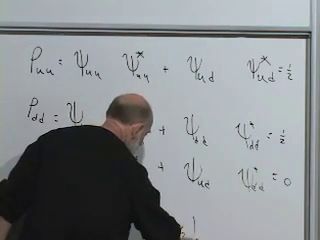
\includegraphics[width=0.76\textwidth]{lecture_08_figure_11.png}
\caption{单态中一个自旋的约化密度矩阵的四个矩阵元。}
\lectureframe{00:55:35}
\end{figure}

\begin{classroomqa}
\lecturetimestamp{00:55:58}
\audiencequestion{单自旋约化态的熵是多少？}
\lecturerresponse{它的两个本征值都是\(1/2\)，所以
\[
S_1=-2\left(\frac12\log\frac12\right)=\log 2.
\]
这是二态子系统所能具有的最大熵。表征最大混合态的是相等的\emph{本征值}，而不是任意基下相等的矩阵元。}
\end{classroomqa}

自旋期望值沿每个轴都为零：
\begin{equation}
\expect{\bm{\sigma}\cdot\hat{\bm n}}
=\operatorname{Tr}\!\left(
\rho_1\,\bm{\sigma}\cdot\hat{\bm n}
\right)
=\frac12\operatorname{Tr}
\left(\bm{\sigma}\cdot\hat{\bm n}\right)
=0.
\end{equation}

\begin{classroomqa}
\lecturetimestamp{00:58:37}
\audiencequestion{为什么\(\bm{\sigma}\cdot\hat{\bm n}\)的迹对每个方向都为零？}
\lecturerresponse{每个泡利矩阵都是无迹的。由于\(\bm{\sigma}\cdot\hat{\bm n}=n_1\sigma_1+n_2\sigma_2+n_3\sigma_3\)，迹的线性性使得对每个单位矢量\(\hat{\bm n}\)结果都为零。因此，自旋沿任意选定轴被找到为平行或反平行的概率相等。}
\end{classroomqa}

整个粒子对具有确定的纯态且熵为零。任一自旋本身都是最大混合的。这不是由有缺陷的制备记录造成的无知；它是纠缠所蕴含的局域态。

\section{等振幅乘积态}

现在考虑
\begin{equation}
\ket{\Phi}
=\frac12\left(
\ket{\uparrow\uparrow}
+\ket{\uparrow\downarrow}
+\ket{\downarrow\uparrow}
+\ket{\downarrow\downarrow}
\right).
\end{equation}
所有四个振幅都等于\(1/2\)，因此归一化来自四个\(1/4\)的贡献。对自旋\(2\)求迹得到
\begin{equation}
\rho_1
=
\begin{pmatrix}
\frac12&\frac12\\[2pt]
\frac12&\frac12
\end{pmatrix}.
\end{equation}
它的迹为\(1\)，但是
\begin{equation}
\det\rho_1
=\frac14-\frac14
=0.
\end{equation}

\begin{classroomqa}
\lecturetimestamp{01:02:23}
\audiencequestion{这里，迹和行列式如何确定两个本征值？}
\lecturerresponse{对于一个\(2\times2\)矩阵，本征值之和为迹，本征值之积为行列式。因此\(\lambda_1+\lambda_2=1\)且\(\lambda_1\lambda_2=0\)，这迫使本征值对为\(\{1,0\}\)。约化态是纯态，其熵为零。}
\end{classroomqa}

\begin{classroomqa}
\lecturetimestamp{01:03:18}
\audiencequestion{这两个未纠缠的自旋实际上在做什么？}
\lecturerresponse{它们都沿正\(x\)轴排列。答案可以通过因式分解识别，
\[
\ket{\Phi}
=\frac{\ket{\uparrow}+\ket{\downarrow}}{\sqrt2}
\otimes
\frac{\ket{\uparrow}+\ket{\downarrow}}{\sqrt2},
\]
或通过计算泡利期望值从实验上确定。}
\end{classroomqa}

对于\(z\)分量，
\begin{equation}
\sigma_3=
\begin{pmatrix}
1&0\\[2pt]
0&-1
\end{pmatrix},
\qquad
\operatorname{Tr}(\rho_1\sigma_3)=0.
\end{equation}
对于\(x\)分量，
\begin{equation}
\sigma_1=
\begin{pmatrix}
0&1\\[2pt]
1&0
\end{pmatrix},
\end{equation}
以及
\begin{align}
\rho_1\sigma_1
&=
\begin{pmatrix}
\frac12&\frac12\\[2pt]
\frac12&\frac12
\end{pmatrix}
\begin{pmatrix}
0&1\\[2pt]
1&0
\end{pmatrix}
=
\begin{pmatrix}
\frac12&\frac12\\[2pt]
\frac12&\frac12
\end{pmatrix}, \\
\operatorname{Tr}(\rho_1\sigma_1)&=1.
\end{align}

\begin{figure}[htbp]
\centering
\includegraphics[width=0.70\textwidth]{lecture_08_figure_03.png}
\caption{等幅约化态的\(\sigma_1\)矩阵计算。}
\lectureframe{01:05:13}
\end{figure}

因此\(\expect{\sigma_1}=1\)而\(\expect{\sigma_2}=\expect{\sigma_3}=0\)。将振幅扰动偏离精确因式分解通常会将本征值从\(\{1,0\}\)变为两个非零值。由此产生的小熵度量了少量纠缠。

\section{这是谁的熵？}

刚才计算的熵属于一个子系统。在单态例子中，
\begin{equation}
S(\rho_{12})=0,
\qquad
S(\rho_1)=S(\rho_2)=\log 2.
\end{equation}
整体是纯态，而每个部分是混合态。因此纠缠熵不服从朴素的加性规则\(S_{12}=S_1+S_2\)。对于二分纯态，两个约化密度矩阵具有相同的非零本征值，所以它们的熵相等，尽管整体的熵为零。

\begin{classroomqa}
\lecturetimestamp{01:09:03}
\audiencequestion{是否每个密度矩阵最终都是纠缠密度矩阵？}
\lecturerresponse{在操作层面上，人们可以描述普通的不确定性，而不追踪是什么承载了缺失的记录。如果制备装置、环境或观察者被包含在内，这种不确定性通常可以被视为与未观测自由度的纠缠。在数学上这个想法是精确的：每个密度矩阵都允许在一个更大的希尔伯特空间上进行纯化，尽管这种纯化并不唯一地确定物理制备历史。}
\end{classroomqa}

\section{从离散经典运动到量子运动}

我们现在暂时离开纠缠，来问状态如何随时间变化。对于一个具有有限多个构型的经典系统，可逆演化是一个置换。每个状态有一个后继和一个前驱；运动分解为循环。

\begin{figure}[htbp]
\centering
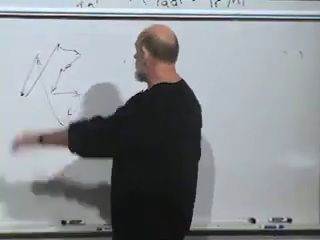
\includegraphics[width=0.70\textwidth]{lecture_08_figure_12.png}
\caption{经典可逆演化由离散构型之间的箭头表示。}
\lectureframe{01:11:40}
\end{figure}

\begin{classroomqa}
\lecturetimestamp{01:11:51}
\audiencequestion{如果构型是离散的，为什么时间步也必须是离散的？}
\lecturerresponse{一个严格经典的两态模型不包含连续路径可以经过的中间构型。缓慢转动一枚物理硬币会引入其朝向作为一个额外的连续坐标，因此它不再是两构型模型。量子两态系统则不同：即使一个正交归一基只有两个成员，其希尔伯特空间也包含一个连续的叠加态族。}
\end{classroomqa}

一个自旋\(\tfrac12\)态可以通过叠加从\(\ket{\uparrow}\)连续旋转到\(\ket{\downarrow}\)。有限维并不意味着状态向量的集合有限。这允许离散量子系统中的连续时间演化。

可逆的微观动力学也保持区分性。两个不同的经典初始条件不会合并为一个微观状态，因为那将抹去哪个初始条件发生了。在哈密顿力学中，这种可逆性伴随着刘维尔定理：相空间体积守恒。

\begin{classroomqa}
\lecturetimestamp{01:15:26}
\audiencequestion{那么非线性分岔中，多个初始条件趋近同一稳态的情况呢？}
\lecturerresponse{吸引子出现在有效的耗散描述中，其中环境自由度已被丢弃。基本的微观哈密顿演化仍然是可逆的；信息可能被转移到未观测的变量，但不同的完整状态不会字面地变成一个完整状态。}
\end{classroomqa}

量子陈述是幺正性。正交的初始态演化为正交的末态，更一般地，每个内积都被保持。

\begin{classroomqa}
\lecturetimestamp{01:16:50}
\audiencequestion{这两个态是否必须受到完全相同的影响？在沿\(x\)方向的磁场中，初始的\(z\)向上态和\(z\)向下态会发生什么？}
\lecturerresponse{同一个演化算符必须作用于这两个态。在横向磁场中，两个自旋进动，但它们的布洛赫矢量始终相反，态矢量始终正交。施加不同的外部历史，就等于在比较不同的演化算符。}
\end{classroomqa}

\section{线性与幺正性}

量子时间演化的第一条原理是线性性：
\begin{equation}
\ket{\psi(t)}=U(t)\ket{\psi(0)}.
\end{equation}
该算符依赖于所经过的时间，并满足
\begin{equation}
U(0)=I.
\end{equation}
与量子力学本身的线性性一样，这条规则由其经验上的成功所证成。

\begin{figure}[htbp]
\centering
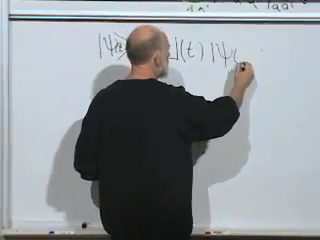
\includegraphics[width=0.70\textwidth]{lecture_08_figure_13.png}
\caption{时刻\(t\)的态由线性算符\(U(t)\)作用于初始态而得到。}
\lectureframe{01:19:00}
\end{figure}

\begin{classroomqa}
\lecturetimestamp{01:19:01}
\audiencequestion{在\(t=0\)时，\(U(t)\)必须是什么？}
\lecturerresponse{它必须是恒等算符。在零经过时间时，对于每一个可能的初始矢量，态都保持不变。}
\end{classroomqa}

第二条原理是内积的保持：
\begin{equation}
\braket{\phi(t)}{\psi(t)}
=\braket{\phi(0)}{\psi(0)}.
\end{equation}
当\(\phi=\psi\)时，这保持归一化，从而保持总概率。当初始态正交时，它保持完全可区分性。对于任意态，它保持它们全部的几何关系。

左矢按照下式演化
\begin{equation}
\bra{\phi(t)}
=\bra{\phi(0)}U^\dagger(t),
\end{equation}
因此
\begin{align}
\braket{\phi(t)}{\psi(t)}
&=\bra{\phi(0)}U^\dagger(t)U(t)\ket{\psi(0)} \\
&=\braket{\phi(0)}{\psi(0)}.
\end{align}
由于这一等式对每一对初始矢量都成立，
\begin{equation}
\boxed{U^\dagger(t)U(t)=I}.
\end{equation}

\begin{figure}[htbp]
\centering
\includegraphics[width=0.74\textwidth]{lecture_08_figure_04.png}
\caption{右矢演化、左矢演化，以及导致\(U^\dagger U=I\)的内积条件。}
\lectureframe{01:23:30}
\end{figure}

\begin{classroomqa}
\lecturetimestamp{01:22:10}
\audiencequestion{为什么左矢获得的是\(U^\dagger\)而不是\(U\)？}
\lecturerresponse{取厄米共轭会颠倒因子的顺序，并把每个算符替换为其厄米共轭：
\[
\bigl(U\ket{\phi}\bigr)^\dagger
=\bra{\phi}U^\dagger.
\]
这正是为了一致的内积所必需的对偶作用。}
\end{classroomqa}

\begin{classroomqa}
\lecturetimestamp{01:24:34}
\audiencequestion{如果\(U\)只是一个复数，那么\(U^\dagger U=1\)意味着什么？}
\lecturerresponse{那将意味着\(|U|=1\)，所以\(U=e^{i\theta}\)位于单位圆上。幺正矩阵是纯相位的算符类比：它保持长度和内积。}
\end{classroomqa}

\section{无穷小演化与哈密顿量}

设\(\epsilon\)为一个非常小的时间间隔。由于\(U(0)=I\)，写出一阶展开
\begin{equation}
U(\epsilon)=I-i\epsilon h+O(\epsilon^2).
\end{equation}
负号以及\(i\)这个因子是方便的约定。取厄米共轭得到
\begin{equation}
U^\dagger(\epsilon)
=I+i\epsilon h^\dagger+O(\epsilon^2).
\end{equation}
幺正性于是要求
\begin{align}
I
&=U^\dagger(\epsilon)U(\epsilon) \\
&=\left(I+i\epsilon h^\dagger\right)
\left(I-i\epsilon h\right)+O(\epsilon^2) \\
&=I+i\epsilon(h^\dagger-h)+O(\epsilon^2).
\end{align}
一阶项必须消失：
\begin{equation}
\boxed{h^\dagger=h}.
\end{equation}
无穷小生成元是厄米的。

\begin{figure}[htbp]
\centering
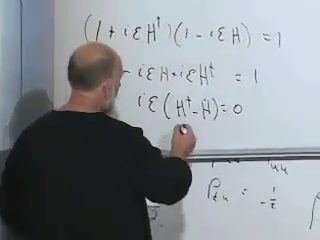
\includegraphics[width=0.76\textwidth]{lecture_08_figure_14.png}
\caption{一阶幺正性迫使无穷小生成元为厄米算符。}
\lectureframe{01:29:35}
\end{figure}

在上述临时约定中，\(h\)具有角频率的量纲。恢复物理单位，定义能量算符
\begin{equation}
H=\hbar h.
\end{equation}
这个厄米算符就是哈密顿量，其本征值是能级。

把无穷小算符作用于一个态：
\begin{equation}
\ket{\psi(\epsilon)}
=\left(I-\frac{i\epsilon}{\hbar}H\right)\ket{\psi(0)}
+O(\epsilon^2).
\end{equation}
减去初始态，除以\(\epsilon\)，并取极限：
\begin{equation}
\frac{\mathrm d}{\mathrm dt}\ket{\psi(t)}
=-\frac{i}{\hbar}H\ket{\psi(t)}.
\end{equation}
等价地，
\begin{equation}
\boxed{
i\hbar\frac{\mathrm d}{\mathrm dt}\ket{\psi(t)}
=H\ket{\psi(t)}
}.
\end{equation}
这就是一般的Schr\"odinger方程。

\begin{figure}[htbp]
\centering
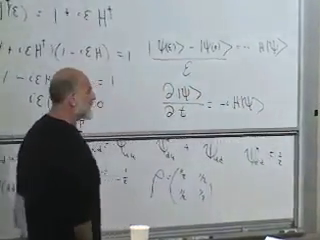
\includegraphics[width=0.76\textwidth]{lecture_08_figure_15.png}
\caption{无穷小差商变成了态的时间导数。}
\lectureframe{01:32:18}
\end{figure}

哈密顿量依赖于物理设置。如果外部磁场或另一种控制发生变化，它可能随时间改变。当设置与时间无关时，\(H\)是一个固定的厄米算符。

\begin{classroomqa}
\lecturetimestamp{01:34:30}
\audiencequestion{内积的保持是否意味着初始未纠缠的系统必须保持未纠缠？}
\lecturerresponse{不。幺正性保持的是完整态矢量之间的内积，而不是所选划分的乘积结构。相互作用哈密顿量可以把一个乘积态变为纠缠态。如果幺正变换做不到这一点，测量就无法使一个系统与一台仪器相关联。}
\end{classroomqa}

\section{熵的单位}

\begin{classroomqa}
\lecturetimestamp{01:35:08}
\audiencequestion{纠缠有诸如焦耳这样的物理单位吗？}
\lecturerresponse{纠缠熵是一种信息度量，而不是能量。使用自然对数时，它以奈特为单位；使用以二为底的对数时，它以比特为单位。两者都是无量纲的计数约定。}
\end{classroomqa}

热力学记号可能会掩盖这一点，因为玻尔兹曼常数在开尔文温度与能量之间进行换算：
\begin{equation}
\expect{K}_{\mathrm{monatomic}}
=\frac32 k_{\mathrm B}T.
\end{equation}
可逆热量关系为
\begin{equation}
\delta Q_{\mathrm{rev}}=T\,\mathrm dS_{\mathrm{th}}.
\end{equation}
如果信息熵为
\begin{equation}
S_{\mathrm{info}}=-\sum_i p_i\log p_i,
\end{equation}
那么传统的热力学熵为
\begin{equation}
S_{\mathrm{th}}=k_{\mathrm B}S_{\mathrm{info}}.
\end{equation}
令\(k_{\mathrm B}=1\)，即以能量单位测量温度，并使熵保持无量纲。于是玻尔兹曼常数被理解为换算因子，而不是一种新的纠缠单位。将玻尔兹曼的统计思想与爱因斯坦1905年关于布朗运动的工作联系起来的历史旁注，并不改变信息论定义。

\section{能量本征态与相位}

\begin{classroomqa}
\lecturetimestamp{01:39:54}
\audiencequestion{为什么厄米生成元\(H\)被等同于能量？}
\lecturerresponse{仅凭幺正性只能证明生成元是厄米的。将其等同于能量是一个额外的物理陈述：能量生成时间平移。对于不含时哈密顿量，支配演化的同一算符是守恒的，其本征值就是定态能级。具体的哈密顿量提供了这一等同的实验内容。}
\end{classroomqa}

普朗克常数与频率之间的关系为
\begin{equation}
E=h\nu=\hbar\omega,
\qquad
\omega=2\pi\nu,
\qquad
h=2\pi\hbar.
\end{equation}

\begin{classroomqa}
\lecturetimestamp{01:40:30}
\audiencequestion{演化方程中应当包含\(h\)、\(\hbar\)，还是多出一个\(2\pi\)因子？}
\lecturerresponse{使用角频率\(\omega\)时，方程为\(E=\hbar\omega\)，而Schr\"odinger方程包含\(\hbar\)。使用普通频率\(\nu\)时，等价关系为\(E=h\nu\)。因子\(2\pi\)完全由\(\omega=2\pi\nu\)和\(h=2\pi\hbar\)解释。}
\end{classroomqa}

假设初始态是能量本征矢量：
\begin{equation}
H\ket{\psi(0)}=E\ket{\psi(0)}.
\end{equation}

\begin{classroomqa}
\lecturetimestamp{01:43:18}
\audiencequestion{如果态仍然是能量本征矢量，这是否意味着它不变化？}
\lecturerresponse{它可能获得一个含时的复因子，并仍以相同本征值作为本征矢量。幺正性将该因子限制为相位。因此，即使右矢在相位上旋转，射线仍是定态的。}
\end{classroomqa}

写出
\begin{equation}
\ket{\psi(t)}=f(t)\ket{\psi(0)}.
\end{equation}

\begin{figure}[H]
\centering
\includegraphics[width=0.70\textwidth]{lecture_08_figure_05.png}
\caption{能量本征态在相差一个标量因子\(f(t)\)的意义下仍沿同一希尔伯特空间方向。}
\lectureframe{01:43:54}
\end{figure}

代入Schr\"odinger方程得到
\begin{align}
i\hbar\frac{\mathrm d f}{\mathrm dt}\ket{\psi(0)}
&=f(t)H\ket{\psi(0)} \\
&=E f(t)\ket{\psi(0)}.
\end{align}
消去公共矢量：
\begin{equation}
\frac{\mathrm d f}{\mathrm dt}
=-\frac{iE}{\hbar}f(t).
\end{equation}
在\(f(0)=1\)下，
\begin{equation}
f(t)=e^{-iEt/\hbar},
\qquad
\ket{\psi(t)}=e^{-iEt/\hbar}\ket{\psi(0)}.
\end{equation}

\begin{figure}[H]
\centering
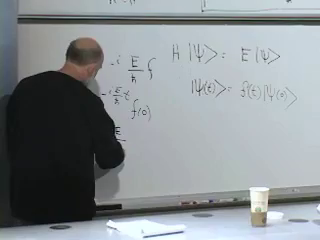
\includegraphics[width=0.76\textwidth]{lecture_08_figure_16.png}
\caption{能量本征值方程及由此得到的相位演化。}
\lectureframe{01:46:10}
\end{figure}

\begin{classroomqa}
\lecturetimestamp{01:45:39}
\audiencequestion{相位\(e^{-iEt/\hbar}\)中\(t\)的系数是什么？}
\lecturerresponse{它是角频率，
\[
\omega=\frac{E}{\hbar}.
\]
等价地，\(E=\hbar\omega\)。实指数系数将描述增长或衰减率；这里的虚指数描述幺正相位旋转。}
\end{classroomqa}

这一相位-频率关系与Schr\"odinger方程是同一时间演化定律的两种形式。该方程是普遍的；自由粒子、势场中的粒子以及磁场中的自旋通过各自的哈密顿量而不同。选择并求解这些哈密顿量是下一步。
